\documentclass{article}

\usepackage[margin=0.8in]{geometry}
\usepackage{listings}
\usepackage{enumerate}
\usepackage{amsmath}
\usepackage{color}
\usepackage{graphicx}

\definecolor{codegreen}{rgb}{0,0.6,0}
\definecolor{codegray}{rgb}{0.5,0.5,0.5}
\definecolor{codepurple}{rgb}{0.58,0,0.82}
\definecolor{backcolour}{rgb}{0.95,0.95,0.92}

\lstdefinestyle{mystyle}{
    backgroundcolor=\color{backcolour},   
    commentstyle=\color{codegreen},
    keywordstyle=\color{magenta},
    numberstyle=\tiny\color{codegray},
    stringstyle=\color{codepurple},
    basicstyle=\footnotesize,
    breakatwhitespace=false,         
    breaklines=true,                 
    captionpos=b,                    
    keepspaces=true,                 
    numbers=left,                    
    numbersep=5pt,                  
    showspaces=false,                
    showstringspaces=false,
    showtabs=false,                  
    tabsize=2
}

\lstset{style=mystyle ,
  language=Python
  % stepnumber=3,    
  % firstnumber=1,
  % numberfirstline=true
}

\title{6.036 Project 3}
\author{Jonathan Garcia-Mallen}
\date{2 May 2016}
\begin{document}
\maketitle

% They want **SINGLE** pdf containing all our answers, code, and graphs. 

\section*{ Part 1: Warm up}
\subsection*{1.a: K-means}
    
    \begin{center}
      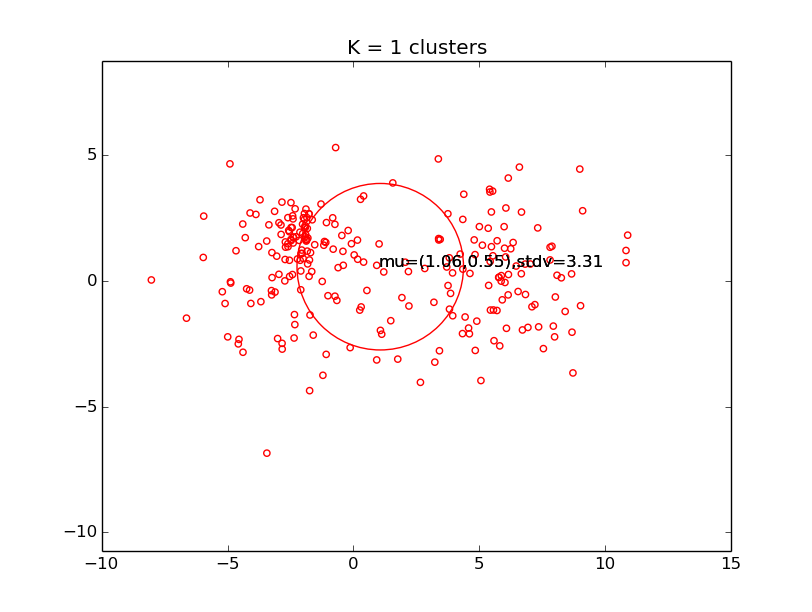
\includegraphics[scale=0.4]{sec1a_k1.png}
      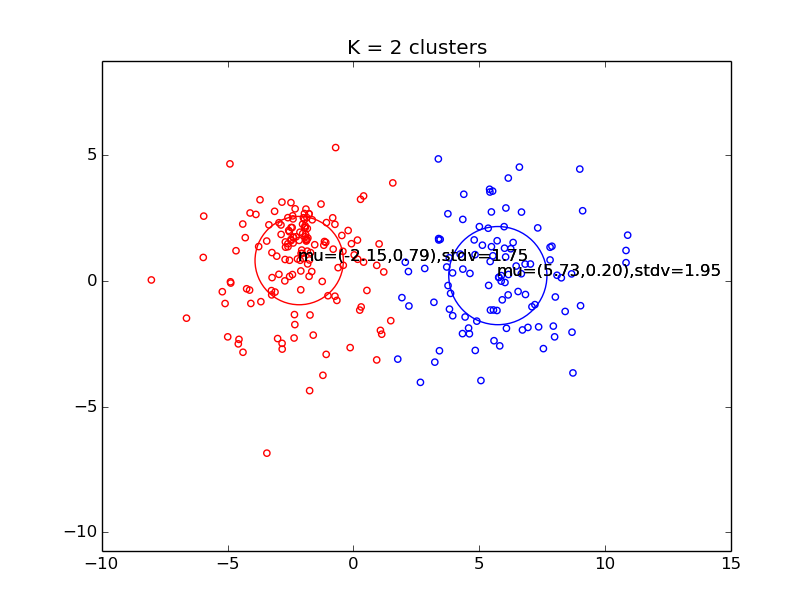
\includegraphics[scale=0.4]{sec1a_k2.png} 
      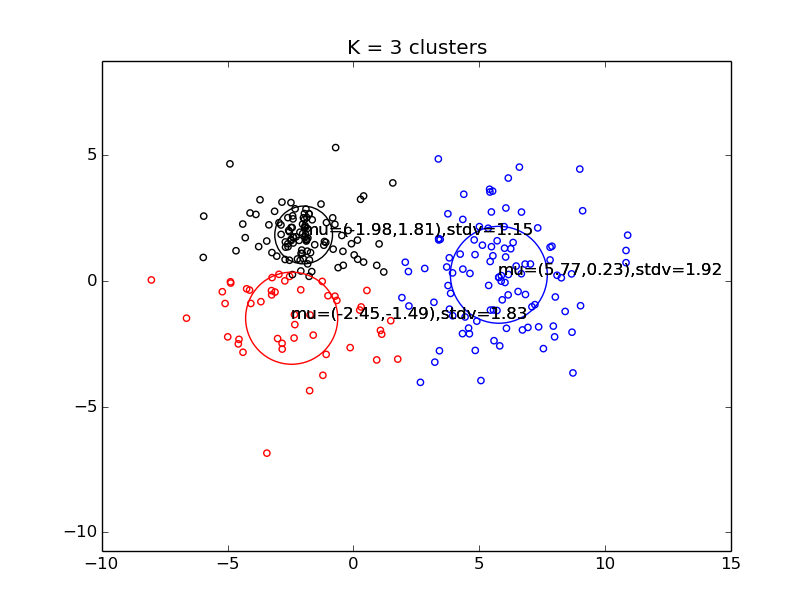
\includegraphics[scale=0.4]{sec1a_k3.png}  
      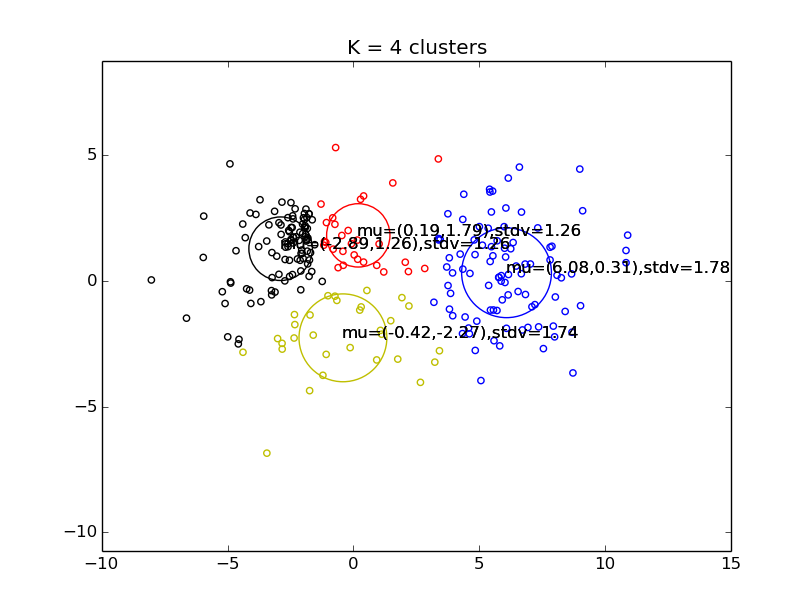
\includegraphics[scale=0.4]{sec1a_k4.png} \\
    \end{center}
     
    Piazza post @609 states to only include code for the skeleton functions explicitly asked to complete.
    The only code for section 1.a is in \texttt{main.py}. 
    The corresponding python snippet, and anything else only found in \texttt{main.py}, will not be copied to this document.

\pagebreak
\subsection*{1.b: Implementing the EM Algorithm}  The routines \texttt{Estep}, \texttt{Mstep}, and \texttt{mixGauss} are all implemented in this section. We also verify \texttt{Estep} here by ensuring a single iteration on the toy data returns $-1331.67489$ as the log-likelihood. My verification in \texttt{main.py} returns $-1331.67489246$ as the log-likelihood.

\subsubsection*{Code for Expectation Step: }
    \begin{lstlisting}
def Estep(X,K,Mu,P,Var):
    n,d = np.shape(X) # n data points of dimension d
    posterior = np.zeros((n,K)) # posterior probabilities to compute
    LL = 0.0    # the LogLikelihood
    # Write your code here

    # Subtract means from corresponding datapoints and store in a (n,d,K)-shaped array
    # Extend datapoint array into 3D array by repeating the X array K times on axis=2.
    normsSquared  =  X.reshape(n,d,1).repeat(K,2)
    # Same for Mu; repeat n times on axis=2. Then transpose to change shape from (K,d,n) to (n,d,K),
    #     and subtract from the X 3D array
    normsSquared -= Mu.reshape(K,d,1).repeat(n,2).transpose((2,1,0))
    # Take squared norm along axis=1, along the feature dimension, which has dimensionality d.
    #     normsSquared.shape now equals (n,K)
    normsSquared = LA.norm(normsSquared,2,1)**2.0

    # Debugging to see if normsSquared is correct.
    # The squared norm of x0-m0 should equal
    
    # Calculate the Spherical Normal/Gaussian Distribution of the datapoints given Mu and Var.
    # np.diag requires a 1D array; Var is given as 2D array with shape (K,1)
    # Also, all operations with variances here are division, so we take the inverse of Var.
    VarInv = np.diag(Var.reshape(K)**-1.0)
    exparg = np.dot(normsSquared, -VarInv/2.0)
    sphericalNormalDist = np.dot(np.exp(exparg), (VarInv/(2*np.pi))**(d/2.0))

    # P(x|theta) = P(datapoint|features) = the denominator in Bayes' theorem.
    # Expressed here on the diagonal of the nxn obvervationsInv matrix.
    # As this is the denominator, we take the inverse of each element to simply multiply later
    observations = np.dot(sphericalNormalDist, P).reshape(n)
    observationsInv = np.diag(observations**-1.0)

    # Use baye's theorem to calculate the posterior probability for each point to be in a cluster
    posterior = np.dot(np.dot(observationsInv, sphericalNormalDist), np.diag(P.reshape(K)))

    # The log-likelihood is just the sum of the log of the observations.
    LL = np.sum(np.log(observations))
    
    return (posterior,LL)
\end{lstlisting}
\pagebreak
\subsubsection*{Code for Maximization Step: }
    \begin{lstlisting}
def Mstep(X,K,Mu,P,Var,post):
    n,d = np.shape(X) # n data points of dimension d

    # Write your code here
    # Effective number of points assigned to cluster corresponding
    # to index along cluster axis=1 in post
    n_hat = np.sum(post, axis=0)
    P  = 1.0*n_hat.reshape(K,1)/n

    Mu = np.dot(np.diag(n_hat**-1.0), np.dot(post.T,X))

    # Var requires squered norms of the datapoints offset by means.
    # It might be possoble to extract the norms from post. Copy/paste from Estep is easier.
    # If I need to use this a third time, I'll make it its own function. 
    normsSquared  =  X.reshape(n,d,1).repeat(K,2)
    normsSquared -= Mu.reshape(K,d,1).repeat(n,2).transpose((2,1,0))
    normsSquared = LA.norm(normsSquared,2,1)**2.0
        # The shape is now hopefully (n,K).

    # I am still confused as to why Var is an input. Keith doesn't use it, so I won't either.
    # the sum should be along the datapoint axis=0
    Var = np.sum(normsSquared * post, axis=0) * (n_hat**-1.0) / d

    return (Mu,P,Var)
\end{lstlisting}

\subsubsection*{Code for the Mixture of Gaussians }
\begin{lstlisting}
def mixGauss(X,K,Mu,P,Var,estp=Estep,mstp=Mstep):
    n,d = np.shape(X) # n data points of dimension d
    post = np.zeros((n,K)) # posterior probabilities
    
    #Write your code here
    #Use function Estep and Mstep as two subroutines
    
    ll_new, ll_old, LL = np.inf, 0, []
    # Has ll_new increased by more than this moving threshold? If so, loop.
    while abs(ll_new - ll_old) >= 10**-6 * np.abs(ll_new) or  np.isinf(ll_new):
        ll_old = ll_new
        (post, ll_new) = estp(X,K,Mu,P,Var)
        (Mu,P,Var) = mstp(X,K,Mu,P,Var, post)

        LL.append(ll_new)      
        
    LL = np.asarray(LL)

    return (Mu,P,Var,post,LL)
\end{lstlisting}

\subsection*{1.c: Verifying the Implementation} There is no code to post for this section. All relevant code is in \texttt{main.py}. \\
Regarding the issue discussed in Piazza post @572, my implementation does one last iteration after obtaining the log-likelihood in the project instructions. When ran with the toy data, my \texttt{mixGauss} has \texttt{LL[-2] = }$-1138.89248$ rather than \texttt{LL[-1]}.
\pagebreak
\subsection*{1.d: EM compared to K-means} All relevant code is in \texttt{main.py}. Here are the graphs:
    \begin{center}
      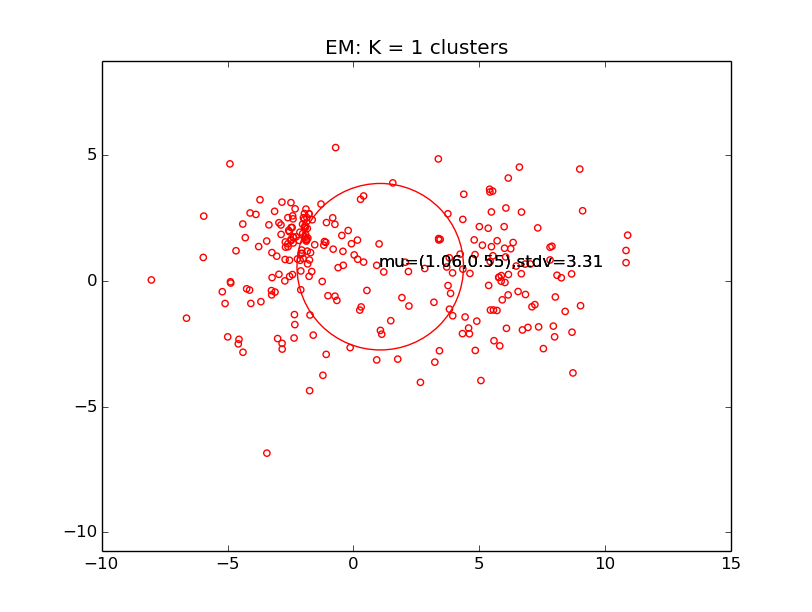
\includegraphics[scale=0.4]{sec1d_k1.png}
      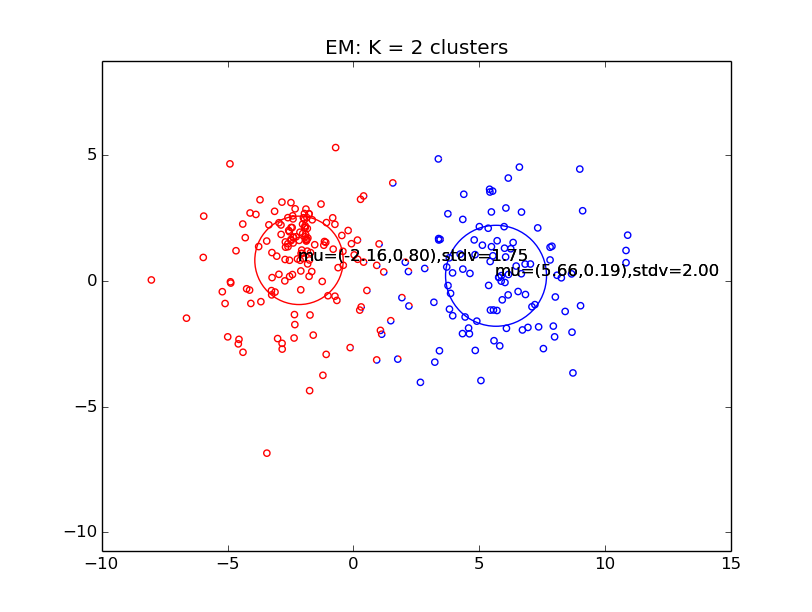
\includegraphics[scale=0.4]{sec1d_k2.png} 
      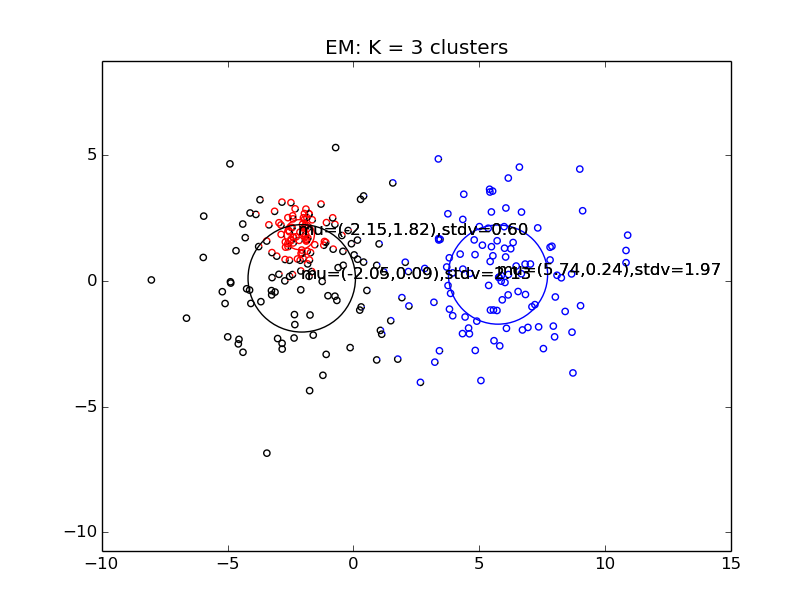
\includegraphics[scale=0.4]{sec1d_k3.png}  
      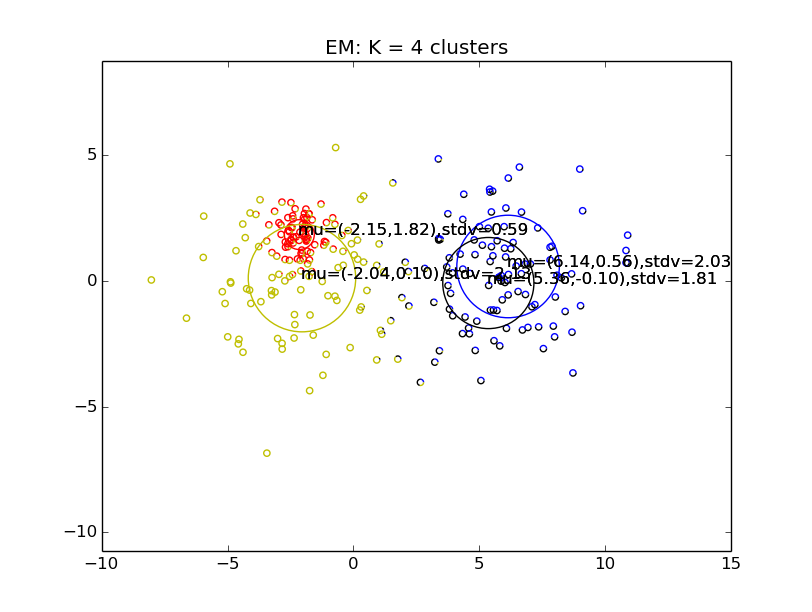
\includegraphics[scale=0.4]{sec1d_k4.png} \\
    \end{center} 
    
    For $K = 1$, EM and K-means are the same. A all points are placed in a single optimal cluster in either algorithm. 

    For $K=2$, the most visible difference lies between the two gaussians in either algorithm.  K-means restricts these datapoints into one of the two distributions. EM instead assigns a proportion of the point to each gaussian, resulting in the red and blue points visible between the distributions. Both gaussians in K-means have a lower standard deviation than those in EM, weightily implying that K-means performed better at $K=2$.

    For $K=3$, the clusters differ even more between either algorithm. We see overlapping gaussians for EM. This reflects the particularly dense region of points near $(-2.1,1.8)$. A human can see that this is likely a single cluster. K-means splits it between its black and red distributions. EM, meanwhile, maintains two clusters with similar means, but very different standard deviations. (For EM, the black standard deviation is $2.13$; difficult to see in the plot.)

    For $K=4$, EM has a pair of overlapping gaussians roughly near $(-2, 1)$ and $(6,0)$, which starts to look more like two clusters. K-means creates four clearly distinct clusters. Again, EM's ability to partially assign points to differenc clusters allows it to have a pair of gaussians that would be clearly better off as one. For EM, the points assigned to the blue and black gaussian are distributed more uniformly than those to the left of the plot. The blue and black means and standard deviations result being very similar. K-means, meanwhile, creates four distinct clusters. These may be more plausible to the eye, depending on the meaning of the underlying data in practice. 

\pagebreak
\subsection*{1.e:  The Bayesian Information Criterion} 
\subsubsection*{Code for the BIC}
\begin{lstlisting}
def BICmix(X,Kset,returnBIC=False,tries=25):
    n,d = np.shape(X)
    #Write your code here

    BIC_best = -np.inf
    K_best = (None, BIC_best)
    for K in Kset:
        # A model with K gausians tries tries tries.
        # Its best log-likelihood from these tries is recorded.
        for i in range(tries):
            # Using randomized means for toy data X
            (Mu,P,Var) = init(X,K)
            # mixGauss returns a tuple. Its last element is a list of ordered LL's. 
            LL = mixGauss(X,K,Mu,P,Var)[-1][-1]

            # Using BIC definition from problem set 5,
            # where a higher BIC implies a better model.
            parameter_count = K*(d+2)-1 # From piazza @571
            BIC_try = LL - 0.5*parameter_count*np.log(n)
            if BIC_try > BIC_best:
                BIC_best = BIC_try
        if K_best[1] < BIC_best:
            K_best = (K, BIC_best)
    if returnBIC:
        return K_best
    else:
        return K_best[0]
\end{lstlisting}
\subsubsection*{Results}

  The best $K$ returned by \texttt{BICmix} is $K = 3$  with BIC score = $-1169.25891336$.

 The data could easily be clustered with either two or three clusters, depending on whether it makes sense for them to overlap much in the underlying data. It quite possible for two data sources to produce points with same mean and very different variances. One example would be two projectile launchers; both with high precision, one with low accuracy; and you're trying to cluster the points to either launcher. With such situations mind, the BIC has indeed selected the correct number of clusters for the toy data. 
\section*{ Part 2: Mixture models for matrix completion}
\subsection*{2.a: Why?} 
If we had all the values and every $x^{(u)}$ were a complete rating vector, then we would have 
\begin{equation*}
  P(x^{(u)}|\theta) = \sum^{K}_{j=1}\pi_jN(x^{(u)} ;\mu^{(j)},\sigma_j^2I )
\end{equation*}
Unfortunately, we have left this ideal world for one where the only values we have for $x^{(u)}$ are those corresponding to the indices $i\in C_U$ $x^{(u)}$. 
How does this impact the previous equation?
Each datapoint $x^{(u)}$ becomes the lower-dimensional $x^{(u)}_{C_u}$ in our calculations. 
We ignore these $d-|C_u|$ dimensions for which we have no values.
This implies we must ignore whatever means are in the dimensions we ignore.
Every $\mu^{(j)}$ must be matched to the reduce dimension of $x^{(u)}_{C_u}$.$x^{(u)}_{C_u}$
So, we work with $\mu^{(j)}_{C_u}$ in order for norm of the difference of the datapoints and the means to make sense. 


In general, each Gaussian in a would have its own matrix of variances $\Sigma_{d\times d}^{(j)}$, where each variance corresponds to a Gaussian on a different dimension. 
We assume our data to be independently and identically distributed, so  $\Sigma_{d\times d}^{(j)} = \sigma_j^2I_{d\times d}$. 
This is why we have the matrix $I$ in the above equation. 
However, since we must ignore the entries $x^{(u)}_i : i \notin C_u$, the only variances we can use are those corresponding to the dimensions denoted by $C_u$. Th
Thus, the matrix of variances becomes of dimension $|C_u|\times |C_u|$, resulting in $\sigma_j^2I_{|C_u|\times |C_u|}$. 
Thus, from the fact that we must focus our model on just the observed portion of each datapoint, we have 
\begin{equation*}
  P(x^{(u)}_{C_u}|\theta) = \sum^{K}_{j=1}\pi_jN(x^{(u)}_{C_u} ;\mu_{C_u}^{(j)},\sigma_j^2I_{|C_u|\times |C_u|} )
\end{equation*}
\subsection*{2.b: Estep}
\begin{lstlisting}
def Estep_part2(X,K,Mu,P,Var):
    n,d = np.shape(X) # n data points of dimension d
    post = np.zeros((n,K)) # posterior probabilities to compute
    LL = 0.0    # the LogLikelihood
    
    # By masking x, we keep from worrying about data we don't have.
    X_ma = np.ma.masked_equal(X, 0)
    VarInv = np.diag(Var.reshape(K)**-1.0)

    # The log of probabilities must be extended in the datapoint dimension to be summed
    P_log = np.log(P).reshape(K,1).repeat(n, 1).T
    
    # Calculate the log of the spherical Normal/gaussian distribution
    normsSquared = differenceSquared(X_ma,Mu)
    nonzeroCounts = -(X != 0).sum(1).reshape(n,1)/2.0

    sphericalNormalDist_log  = np.dot(nonzeroCounts,np.log(2*np.pi*Var.T))
    sphericalNormalDist_log += np.dot(normsSquared, -VarInv/2.0)

    # Calculate the log of the observations using advice in project3.pdf
    numerator = P_log + sphericalNormalDist_log
    observation_log = logsumexp(numerator, axis=1).reshape(n,1)

    LL = np.sum(observation_log)
    
    observation_log = observation_log.repeat(K,1)
    post = np.subtract(numerator, observation_log)
    return (np.exp(post),LL)
\end{lstlisting}
\subsection*{2.c: Mstep}
\begin{lstlisting}
def Mstep_part2(X,K,Mu,P,Var,post, minVariance=0.25):
    n,d = np.shape(X) # n data points of dimension d
    
    #Write your code here
    X_ma = np.ma.masked_equal(X, 0)
    indicator = (X != 0)
    nonzeroCounts = indicator.sum(1).reshape(1,n)

    # find the means. This took time, and could be better, but it works. 
    Mu_denom = np.dot(post.T, indicator)
    Mu_numer = np.dot(post.T, X_ma)
    Mu_update = Mu_numer / Mu_denom
    for j in range(K):
        for i in range(d):
            if Mu_denom[j,i] < 1:
                Mu_update[j,i] = Mu[j,i]
    Mu = Mu_update
    
    # Cluster Probabilies
    P = post.sum(0)/float(n)

    # find the variances
    Var_numer = (post * differenceSquared(X_ma, Mu)).sum(0).reshape(K,1)
    Var_denom = np.dot(nonzeroCounts,post).T
    Var = Var_numer / Var_denom
    for variance in np.nditer(Var, op_flags=['readwrite']):
        if variance < minVariance:
            variance[...] = minVariance
    
    return (Mu,P,Var)
\end{lstlisting}
\subsection*{2.d: Finishing the EM implementation, mixGauss\_part2}
We aren't required to turn in any code for debugging, and we don't need to report any data, so here is my \texttt{mixGauss\_part2} 
\begin{lstlisting}
def mixGauss_part2(X,K,Mu,P,Var):
    n,d = np.shape(X) # n data points of dimension d
    post = np.zeros((n,K)) # posterior probs tbd
    
    #Write your code here
    #Use function Estep and Mstep as two subroutines
    return mixGauss(X,K,Mu,P,Var,Estep_part2,Mstep_part2)
\end{lstlisting}
\subsection*{2.e: Implementation Validation}
After running the monotonicity verifyier in \texttt{main.py} and storing the resulting list of log-likelihoods:
\begin{verbatim}
>>> print LL[-1]
-1389515.88823
>>> 
\end{verbatim}
The note from section 1.c still stands.
\subsection*{2.f: How to fill X}
\begin{center}$x_i^{(t)} = \sum_{j=1}^K \pi_j \mu_i^{(j)}$\end{center}

\subsection*{2.g: Filling it all up}
\begin{lstlisting}
def fillMatrix(X,K,Mu,P,Var):
    n,d = np.shape(X)
    Xnew = np.copy(X)
    print '(n,K,d)',  (n,K,d)
    #Write your code here
    for t in range(n):
        for i in range(d):
            if Xnew[t,i] == 0:
                Xnew[t,i] = np.dot(P.reshape(K), Mu.T[i])        
    return Xnew
\end{lstlisting}
\end{document}

